\PassOptionsToPackage{unicode=true}{hyperref} % options for packages loaded elsewhere
\PassOptionsToPackage{hyphens}{url}
%
\documentclass[ignorenonframetext,]{beamer}
\setbeamertemplate{caption}[numbered]
\setbeamertemplate{caption label separator}{: }
\setbeamercolor{caption name}{fg=normal text.fg}
\beamertemplatenavigationsymbolsempty
\usepackage{lmodern}
\usepackage{amssymb,amsmath}
\usepackage{ifxetex,ifluatex}
\usepackage{fixltx2e} % provides \textsubscript
\ifnum 0\ifxetex 1\fi\ifluatex 1\fi=0 % if pdftex
  \usepackage[T1]{fontenc}
  \usepackage[utf8]{inputenc}
  \usepackage{textcomp} % provides euro and other symbols
\else % if luatex or xelatex
  \usepackage{unicode-math}
  \defaultfontfeatures{Ligatures=TeX,Scale=MatchLowercase}
\fi
% use upquote if available, for straight quotes in verbatim environments
\IfFileExists{upquote.sty}{\usepackage{upquote}}{}
% use microtype if available
\IfFileExists{microtype.sty}{%
\usepackage[]{microtype}
\UseMicrotypeSet[protrusion]{basicmath} % disable protrusion for tt fonts
}{}
\IfFileExists{parskip.sty}{%
\usepackage{parskip}
}{% else
\setlength{\parindent}{0pt}
\setlength{\parskip}{6pt plus 2pt minus 1pt}
}
\usepackage{hyperref}
\hypersetup{
            pdftitle={Interim Monitoring: Pitfalls and Recommendations},
            pdfauthor={Dave Harrington},
            pdfborder={0 0 0},
            breaklinks=true}
\urlstyle{same}  % don't use monospace font for urls
\newif\ifbibliography
\usepackage{graphicx,grffile}
\makeatletter
\def\maxwidth{\ifdim\Gin@nat@width>\linewidth\linewidth\else\Gin@nat@width\fi}
\def\maxheight{\ifdim\Gin@nat@height>\textheight\textheight\else\Gin@nat@height\fi}
\makeatother
% Scale images if necessary, so that they will not overflow the page
% margins by default, and it is still possible to overwrite the defaults
% using explicit options in \includegraphics[width, height, ...]{}
\setkeys{Gin}{width=\maxwidth,height=\maxheight,keepaspectratio}
% Prevent slide breaks in the middle of a paragraph:
\widowpenalties 1 10000
\raggedbottom
\setbeamertemplate{part page}{
\centering
\begin{beamercolorbox}[sep=16pt,center]{part title}
  \usebeamerfont{part title}\insertpart\par
\end{beamercolorbox}
}
\setbeamertemplate{section page}{
\centering
\begin{beamercolorbox}[sep=12pt,center]{part title}
  \usebeamerfont{section title}\insertsection\par
\end{beamercolorbox}
}
\setbeamertemplate{subsection page}{
\centering
\begin{beamercolorbox}[sep=8pt,center]{part title}
  \usebeamerfont{subsection title}\insertsubsection\par
\end{beamercolorbox}
}
\AtBeginPart{
  \frame{\partpage}
}
\AtBeginSection{
  \ifbibliography
  \else
    \frame{\sectionpage}
  \fi
}
\AtBeginSubsection{
  \frame{\subsectionpage}
}
\setlength{\emergencystretch}{3em}  % prevent overfull lines
\providecommand{\tightlist}{%
  \setlength{\itemsep}{0pt}\setlength{\parskip}{0pt}}
\setcounter{secnumdepth}{0}

% set default figure placement to htbp
\makeatletter
\def\fps@figure{htbp}
\makeatother


\usepackage{amsmath,verbatim}

\usepackage{fancyvrb}
\usepackage{manfnt}
\usepackage[normalem]{ulem}

%\usepackage[colorlinks=true]{hyperref}

\mode<presentation>{\usetheme{Malmoe}}

%\synctex=1

\setbeamertemplate{headline}{}


\setbeamerfont{footline}{size=\scriptsize}
\setbeamerfont{frametitle}{shape=\scshape}
\setbeamertemplate{itemize items}[circle]
\setbeamercovered{transparent}

\setbeamertemplate{navigation symbols}{}
\setbeamertemplate{footline}[frame number]{} 


\definecolor{forest}{rgb}{0, .5, 0}
\definecolor{brick}{rgb}{.5, 0, 0}
\definecolor{darkgreen}{rgb}{0, .5, 0}
\definecolor{darkred}{rgb}{.7, .15, .15}
\definecolor{darkblue}{rgb}{0, 0, .5}
\definecolor{Green}{rgb}{0.2,1,0.2}


\newcommand{\R}{\textsf{R}}
\newcommand{\RStudio}{\textsl{R Studio}}


\usepackage[english]{babel}
%\usepackage{palatino}
\usepackage[T1]{fontenc}


% make all tt fonts bold to look more like Verbatim
\usepackage{lmodern}
\renewcommand\ttfamily{\usefont{T1}{lmtt}{m}{n}}

% Comment these out if you don't want a slide with just the
% part/section/subsection/subsubsection title:
\AtBeginPart{
  \let\insertpartnumber\relax
  \let\partname\relax
  \frame{\partpage}
}
\AtBeginSection{
  \let\insertsectionnumber\relax
 \let\sectionname\relax
 \frame{\sectionpage}
}
\AtBeginSubsection{
  \let\insertsubsectionnumber\relax
  \let\subsectionname\relax
  \frame{\subsectionpage}
}

\title{Interim Monitoring: Pitfalls and Recommendations}
\providecommand{\subtitle}[1]{}
\subtitle{FDA Mini-Symposium on Role of DMCs, Sponsors \& Regulators in the Era of
Breakthrough Therapy and Accelerated Approval in Oncology Clinical
Trials}
\author{Dave Harrington}
\date{2 July 2019}

\begin{document}
\frame{\titlepage}

\hypertarget{design-issues}{%
\section{Design Issues}\label{design-issues}}

\begin{frame}{%
\protect\hypertarget{anticipating-tx-effects}{%
Anticipating Tx effects}}

Inotuzumab Ozogamicin versus Standard Therapy for ALL (NEJM 25 Aug 2016)

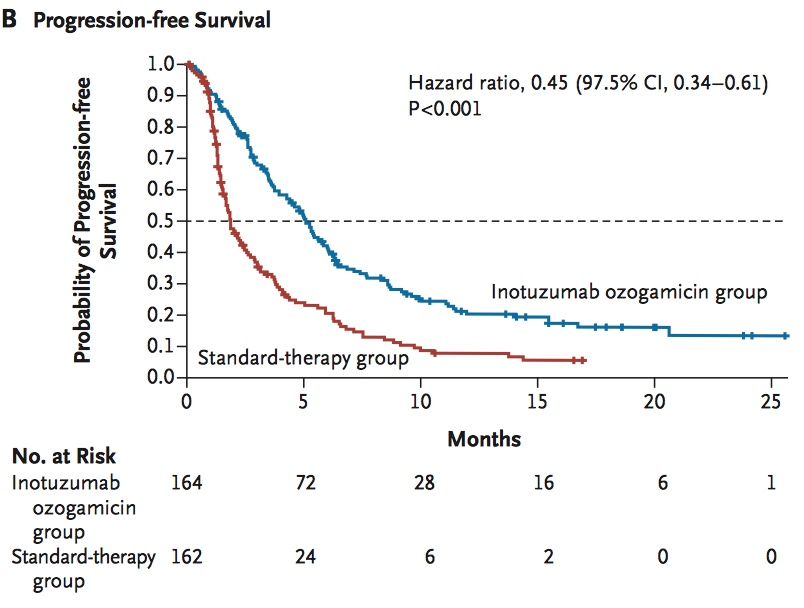
\includegraphics[width=0.75\textwidth,height=\textheight]{./figures/pfs_all.jpeg}

\end{frame}

\begin{frame}{%
\protect\hypertarget{section}{%
}}

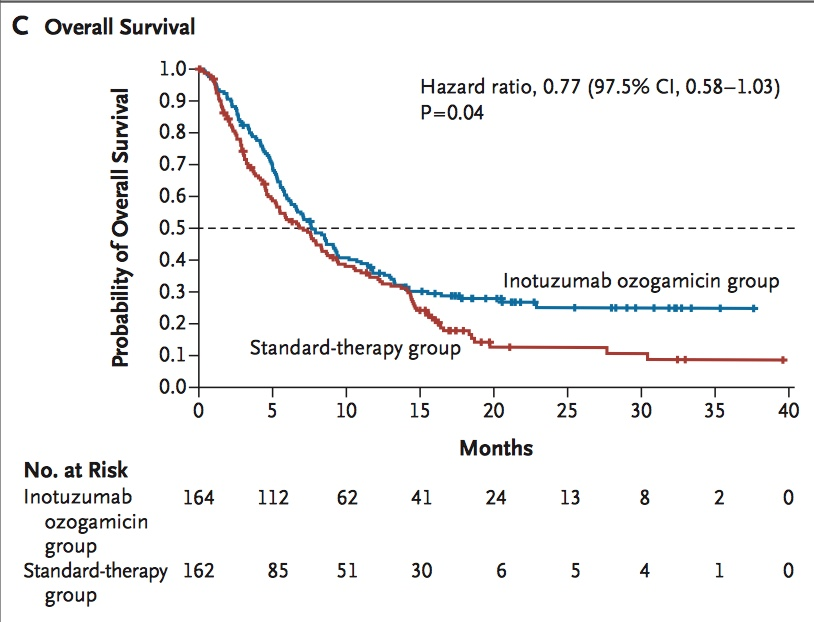
\includegraphics[width=0.75\textwidth,height=\textheight]{./figures/os_all.jpeg}

\end{frame}

\begin{frame}{%
\protect\hypertarget{metastic-prostate-cancer}{%
Metastic prostate cancer}}

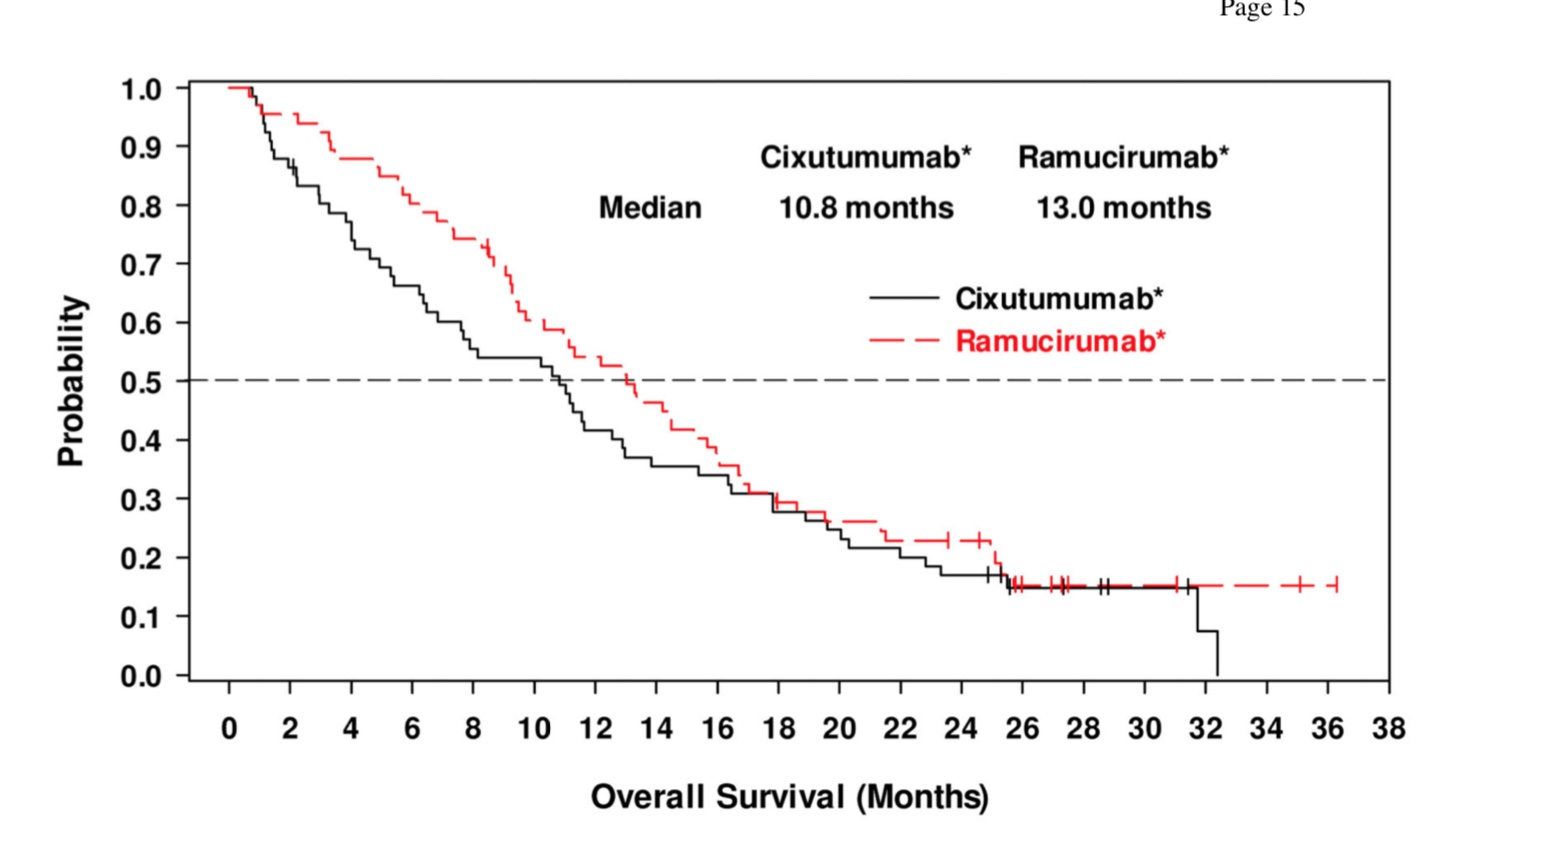
\includegraphics[width=0.8\textwidth,height=\textheight]{./figures/hussain_survival.jpg}

Hussain, et al., Eur J Cancer, Sep 2015

\end{frame}

\begin{frame}{%
\protect\hypertarget{correct-assumptions-may-depend-on-disease-andor-agent}{%
Correct assumptions may depend on disease and/or agent}}

From Alexander, et al., NEJM March 2018

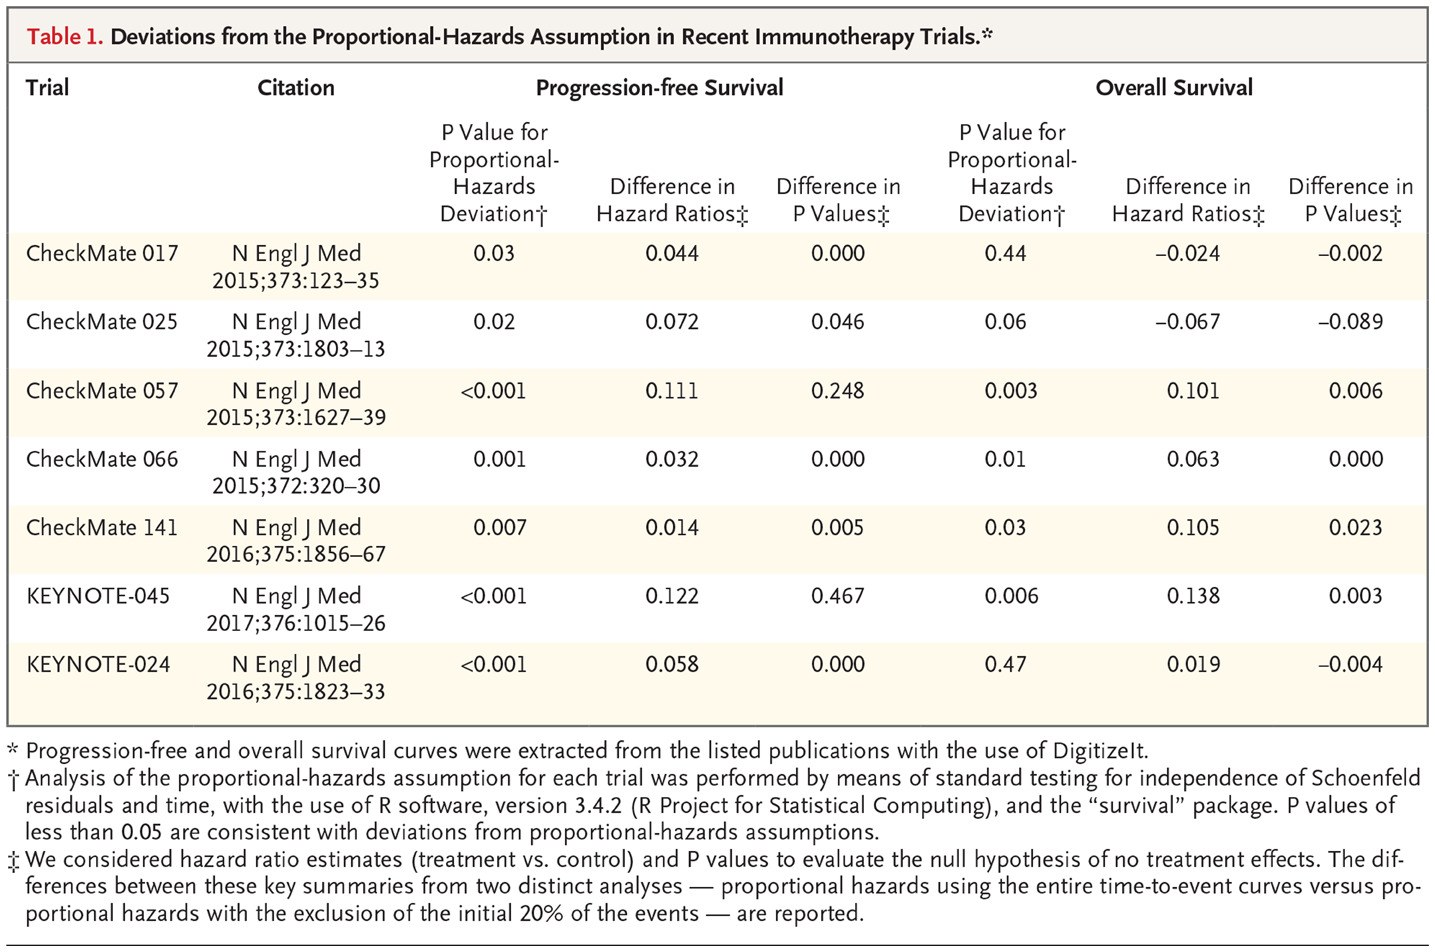
\includegraphics[width=0.9\textwidth,height=\textheight]{./figures/trippa_table.jpg}

\end{frame}

\begin{frame}{%
\protect\hypertarget{substantial-methodology-available}{%
Substantial methodology available}}

Korn and Freidlin, 2018 JCO, Am. J.Bioethics 2011

Freidlin and Korn, Clin Trials, 2009; Cont Clin Trials, 2002

Work presented at Feb 2018 Duke Margolis Workshop

\begin{itemize}
\tightlist
\item
  Oncology Clinical Trials in the Presence of Non-Proportional Hazards
\end{itemize}

\end{frame}

\hypertarget{issues-external-to-the-trial}{%
\section{Issues external to the
trial}\label{issues-external-to-the-trial}}

\begin{frame}{%
\protect\hypertarget{following-the-monitoring-plan-was-the-wrong-thing-to-do}{%
Following the monitoring plan was the wrong thing to do}}

Extracorporeal Membrane Oxygenation ECMO for ARDS (NEJM 24 May 2018)

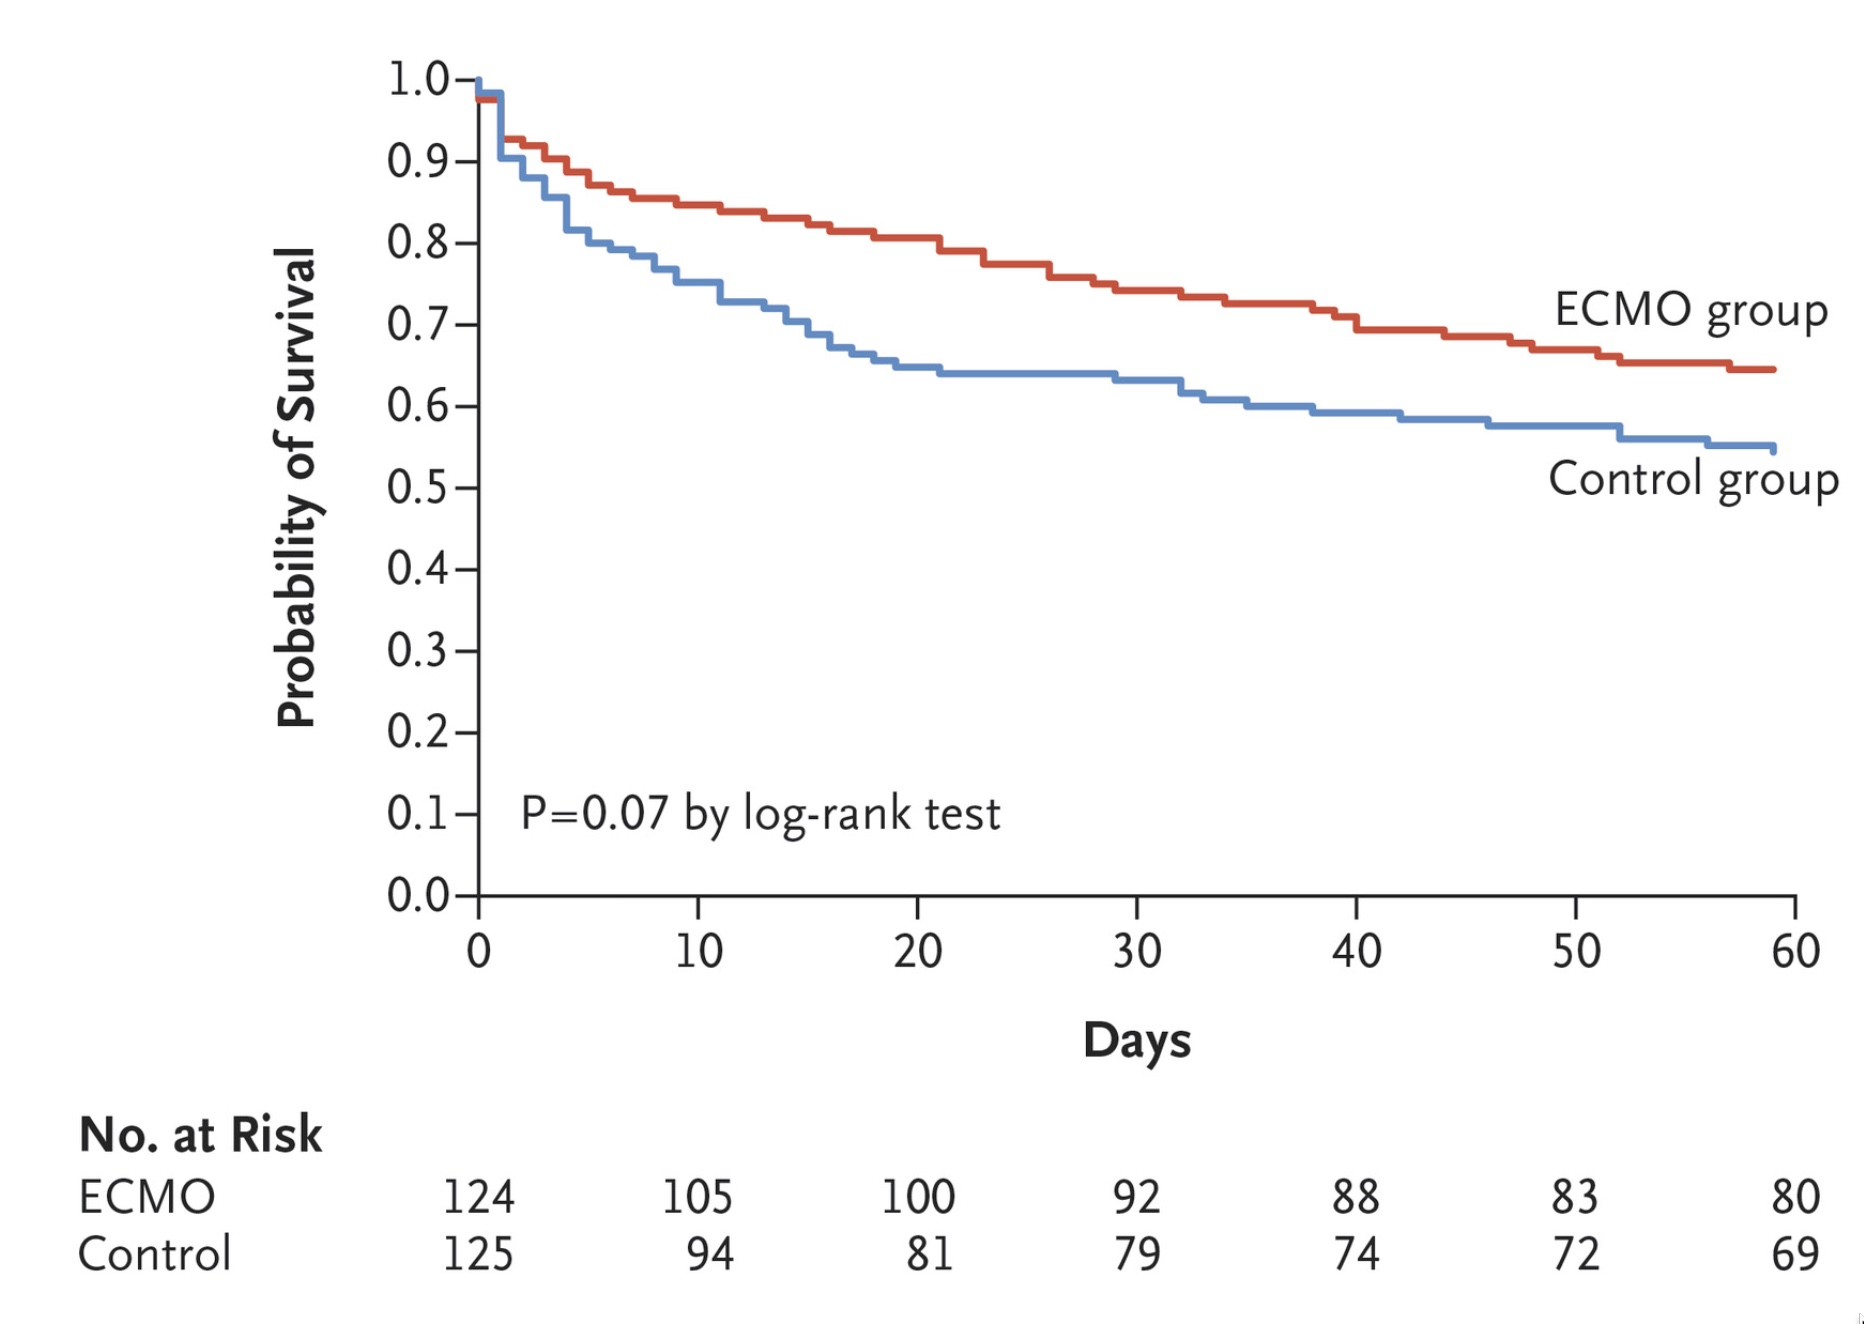
\includegraphics[width=0.75\textwidth,height=\textheight]{./figures/ecmo_survival.jpeg}

Figure 2

\end{frame}

\begin{frame}{%
\protect\hypertarget{ecmo-stopping-rule-figure-s1}{%
ECMO Stopping Rule: Figure S1}}

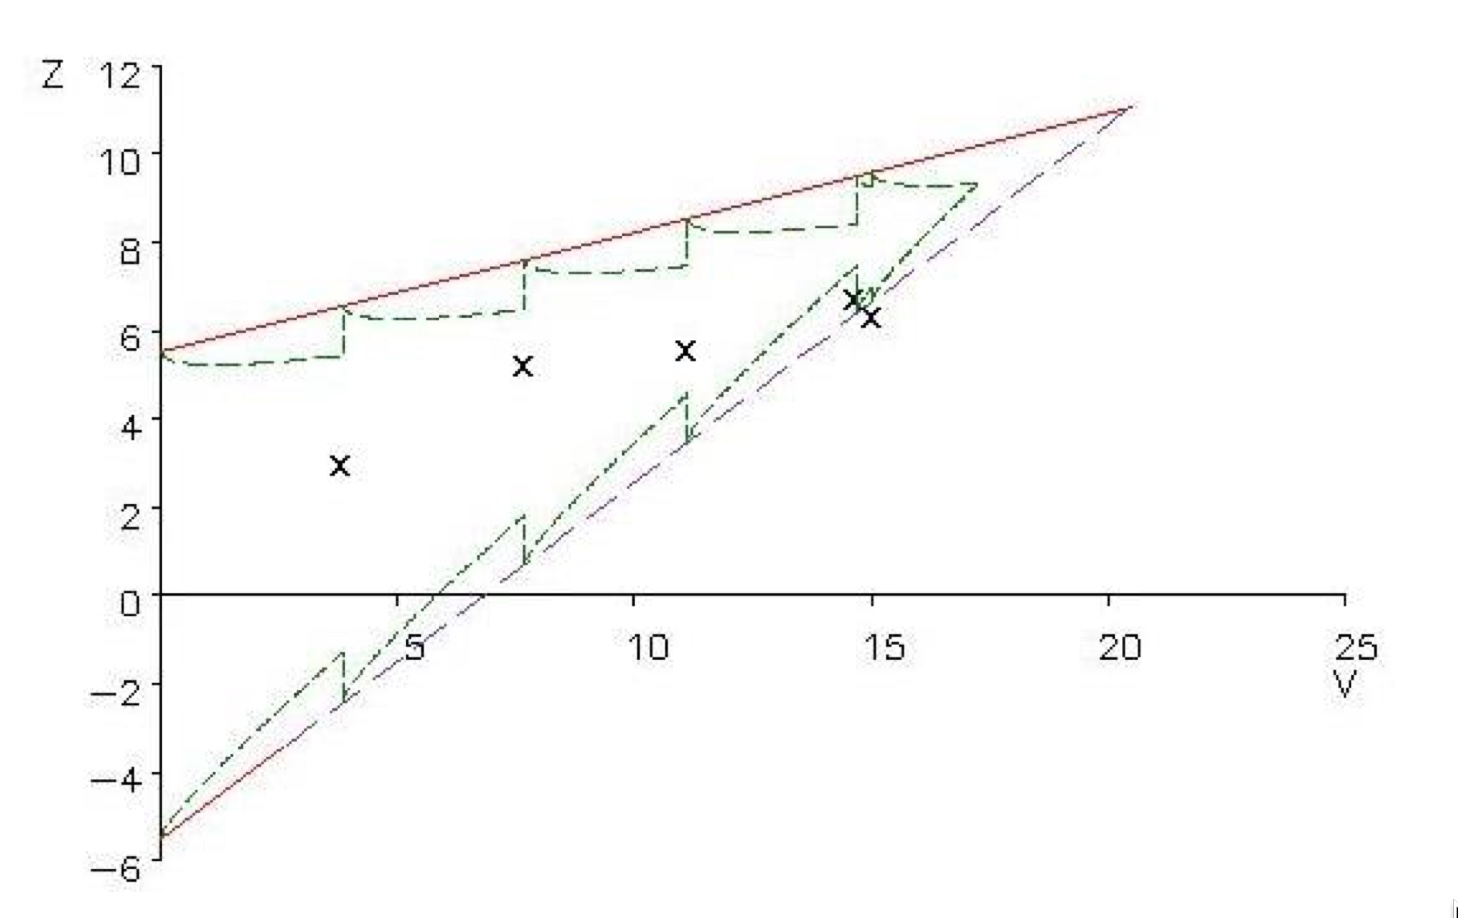
\includegraphics[width=0.7\textwidth,height=\textheight]{./figures/ecmo_monitoring.jpeg}

\begin{itemize}
\item
  Trial stopped for futility at 4th interim analysis, with 240/331
  patients.
\item
  HR 0.70 favoring ECMO, 95\% confidence interval (0.47, 1.04), p = 0.07
\end{itemize}

\end{frame}

\begin{frame}{%
\protect\hypertarget{not-following-the-plan-was-the-right-thing-to-do}{%
Not following the plan was the right thing to do}}

Heart and Lung Transplants from HCV+ Donors (Woolley, et al.,NEJM 25
April 2019)

\begin{itemize}
\item
  Original Design based on Simon two-stage phase II design.
\item
  Amended to modified SPRT to allow continuous monitoring.

  \begin{itemize}
  \tightlist
  \item
    Boundaries for superiority and safety
  \end{itemize}
\end{itemize}

\end{frame}

\begin{frame}{%
\protect\hypertarget{hcv-transplanted-organs}{%
HCV+ Transplanted organs \ldots}}

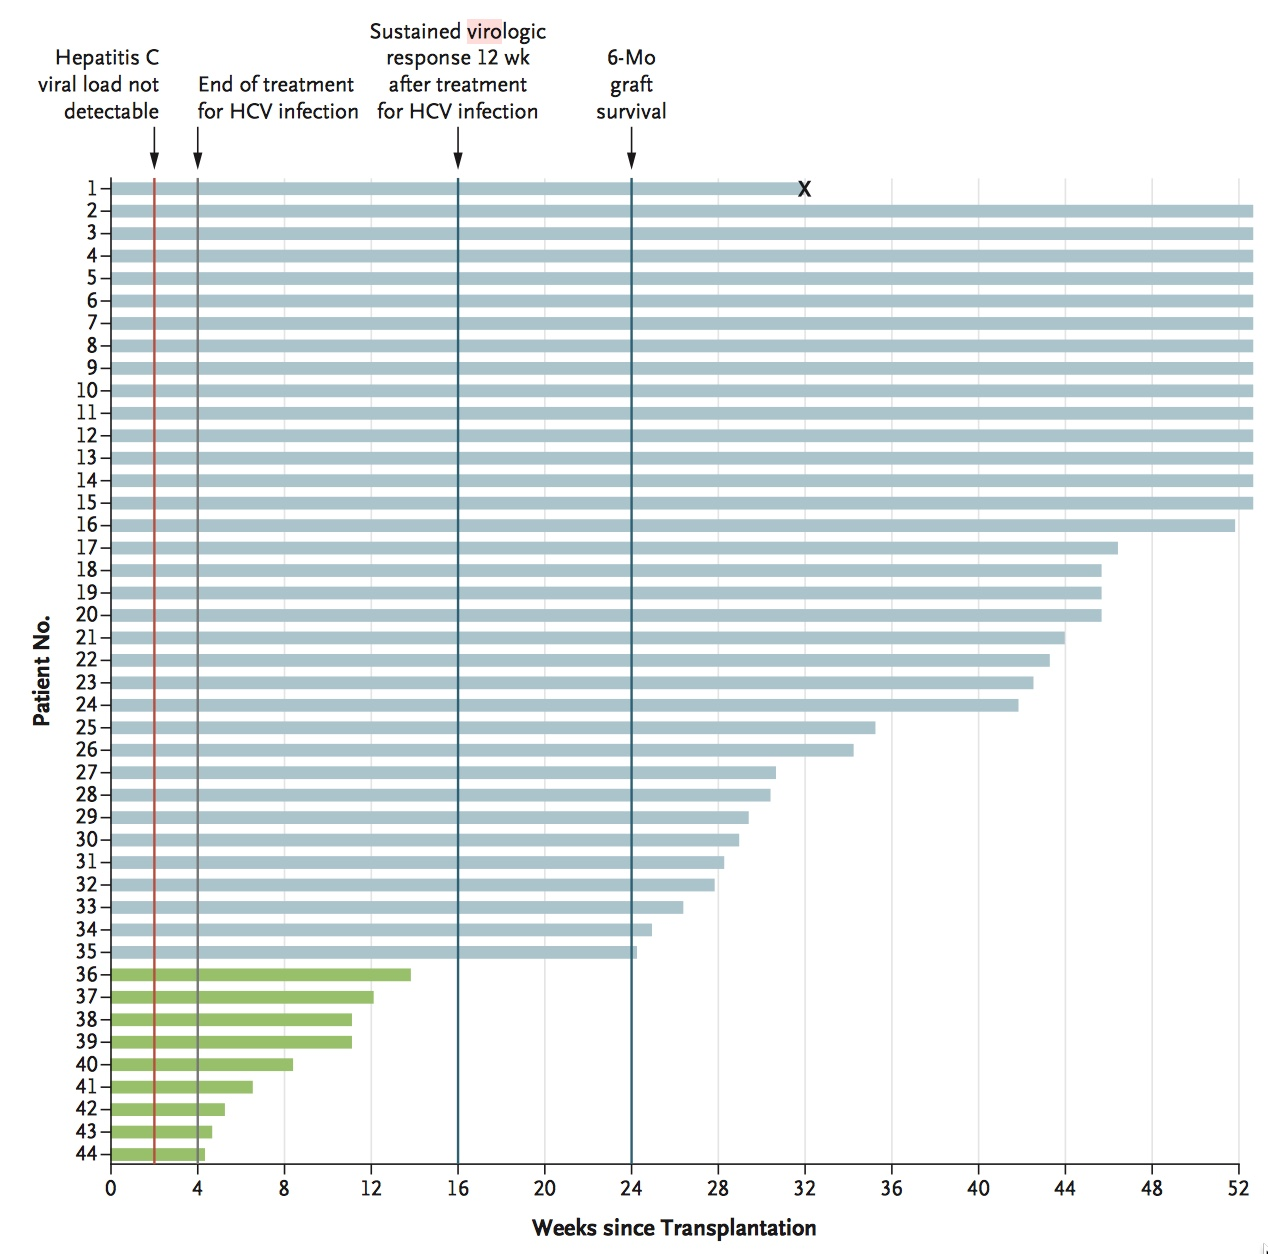
\includegraphics[width=0.68\textwidth,height=\textheight]{./figures/hcv_monitoring.jpeg}

Figure 2: Crossed stopping boundary for efficacy at 13 patients with 6
mo follow-up

\end{frame}

\begin{frame}{%
\protect\hypertarget{recommendationsquestions}{%
Recommendations/Questions}}

\begin{itemize}
\item
  DMC and FDA should probe whether monitoring plan uses

  \begin{itemize}
  \item
    Best available data to anticipate nature of differences.
  \item
    Best available methodology for monitoring
  \end{itemize}
\item
  In the absence of harm, non-significant but positive Tx effects may be
  important.

  \begin{itemize}
  \tightlist
  \item
    Be reluctant to stop when HR favors experimental Tx
  \end{itemize}
\item
  Monitoring plans should incorporate interim sensitivity analyses for
  different types of Tx effects.
\item
  Is a surrogate endpoint risky? (eg, PFS vs OS)
\end{itemize}

\end{frame}

\begin{frame}{%
\protect\hypertarget{recommendations}{%
Recommendations \ldots}}

\begin{itemize}
\item
  DMC should be less literal in executing monitoring plans when faced
  with external information.
\item
  Data sharing between DMCs or between DMC and FDA should be guaranteed
  confidential, including the use of secure communications.
\item
  Does the FDA perspective on interim futility monitoring coincide with
  trials not designed for regulatory approval?
\item
  Should we continue to design around proportional hazards?
\end{itemize}

\end{frame}

\end{document}
